%=========================================================
\chapter{Modelo Estático}	
\label{cap:modeloEstatico}

	Este capítulo describe las reglas de modelado y decisiones de Arquitectura tomadas en el sistema, sin tener en cuenta la acción del tiempo sobre el mismo.

%---------------------------------------------------------
\section{Modelado de Subsistemas}

    Se utilizará la Arquitectura de Tres Capas, debido a su estabilidad y efectividad probada para construir plataformas web como la que pretendemos utilizar.
    Facilita también encontrar problemas, al limitar la comunicación entre capas, y si a eso sumamos el hecho de que facilita la distribución de trabajo al estar bien definidas y modularizadas cada una de las capas, resulta ser bastante sólida y acorde a nuestras necesidades en el proyecto.
    
    \begin{figure}[htbp!]
    	\begin{center}
    		\fbox{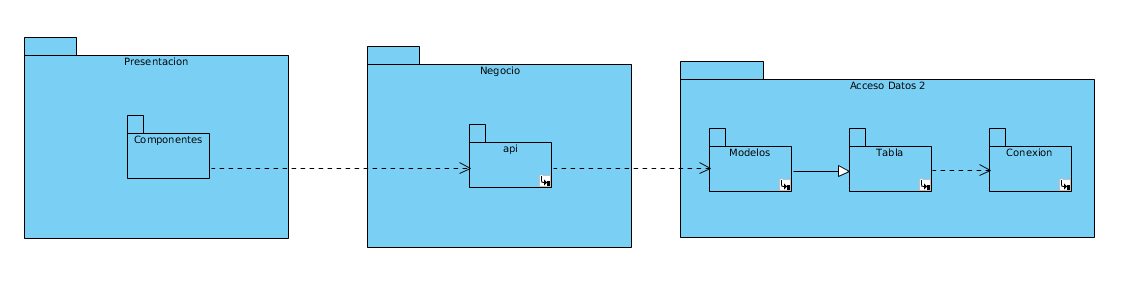
\includegraphics[width=.8\textwidth]{tlato-images/Subsistemas.png}}
    		\caption{Arquitectura del sistema.}
    		\label{fig:subsistemas}
    	\end{center}
    \end{figure}
    
    \subsection{Capa de Acceso a Datos}
    También llamada Capa de Persistencia, esta capa se encarga de guardar los datos. Será donde se gestione todo lo relativo a la base de datos y a la creación, edición y borrado de datos de ésta, así como proporcionar los datos necesarios a la Capa de Negocio.
    Cabe mencionar que sólo puede comunicarse con la Capa de Negocio.
    
    \subsection{Capa de Negocio}
    En esta capa se gestionan los procesos importantes de la lógica de la aplicación. Todo lo relacionado con lógica de negocio, reglas de negocio y cómo se controla el flujo de datos dentro del sistema para cada usuario irá en este sub-sistema.
    
    \subsection{Capa de Presentación}
    En esta capa se manejará la interfaz del usuario. Su función es pasarle las acciones que realice el usuario a la capa de negocio, para que ésta ejecute las operaciones necesarias

%---------------------------------------------------------
\section{Modelado de Módulos}	

    En esta sección se describirán los módulos de los que estarán compuestos cada uno de los subsistemas descritos en la seccion anterior, explicando cuales son las características y responsabilidades de cada uno de ellos. 
    
    
    \subsection{Módulo del subsistema acceso a datos}
    \begin{figure}[htbp!]
    	\begin{center}
    		\fbox{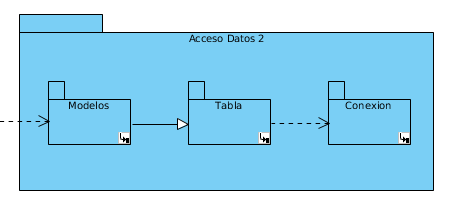
\includegraphics[width=.7\textwidth]{tlato-images/acceso_datos}}
    		\caption{Estructura del modulo de Acceso a Datos}
    		\label{fig:packagedatos}
    	\end{center}
    \end{figure}
        
    En la figura~\ref{fig:packagedatos} se detalla el contenido de la Capa de Acceso a Datos. Se encuentra dividida modularmente en tres paquetes, de tal forma que se minimice la repetición de código, y el aceso a los datos sea limpio y seguro. Los paquetes son: \\
    \begin{itemize}
        \item Conexión, el cual contiene las constantes de conexión a base de datos, así como las operaciones fundamentales de realización de consultas.
        \item Tabla, la cual, usando la configuración del paquete anterior, contiene las instrucciones que usan la mayoría de las tablas, como Insertar, Editar, Eliminar y listar.
        \item Modelos, paquete que hereda de Tabla, y ejecuta las instrucciones, afectando a los campos personalizados de cada tabla, revolviendo generalmente arreglos u objetos para ser utilizados por la capa de Negocio, o recibiendo datos de ella.
    \end{itemize}
        
        
    \subsection{Modulo de Negocios}
    \begin{figure}[htbp!]
    	\begin{center}
    		\fbox{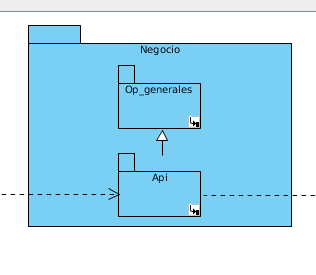
\includegraphics[width=.3\textwidth]{tlato-images/negocio}}
    		\caption{Estructura del modulo de Negocio}
    		\label{fig:negocio}
    	\end{center}
    \end{figure}
        
    En la figura~\ref{fig:negocio} se muestran detalles estructurales de la Capa de Negocio. \\
    En esta capa se maneja toda la lógica de negocio, y debido al estilo estructural que hemos dado al proyecto, por cada elemento en el paquete de Datos.Modelos existirá un elemento en el paquete API. La forma de operar de esta carpeta es escuchar por peticiones de la capa de Presentación, a partir de ellas realizar peticiones a la capa de Acceso a Datos, y devolverle datos a la capa de presentación en formato JSON. Se estructura en:
    \begin{itemize}
        \item op\_generales: Esta contiene los manejadores para las operaciones generales de procesar peticiones [GET y POST] y enviar respuestas. Es una generalizacion de los objetos del paquete API.
        \item API: Contiene extensiones a las operaciones desarrolladas por op\_generales, añadiendo funcionalidades que esta no cubre de acuerdo a la necesidad de cada objeto.
    \end{itemize}
    
    
    \subsection{Modulo de Presentacion}
    \begin{figure}[htbp!]
    	\begin{center}
    		\fbox{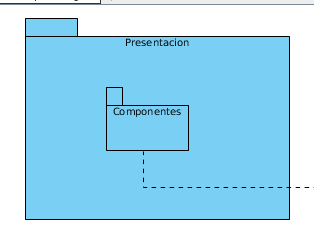
\includegraphics[width=.3\textwidth]{tlato-images/presentacion}}
    		\caption{Estructura del modulo de Presentacion}
    		\label{fig:presentacion}
    	\end{center}
    \end{figure}
        
    La figura ~\ref{fig:presentacion} detalla el módulo de presentación, el cual contiene únicamente una carpeta, llamada componentes. \\
    La ideología se basa en que cada trozo de pantalla corresponde a un componente, y éste puede ser reutilizado en múltiples pantallas, maximizando, de nuevo, la re-utilización del código, y haciendo que dichos componentes funcionen exactamente de la misma manera en cada sitio de donde sean llamados.
%---------------------------------------------------------
\section{Modelado de Clases}	

\subsection{Clases del modelo Datos.Conexion}
    Datos del Modulo Conexion
    
    \begin{figure}[htbp!]
    	\begin{center}
    		\fbox{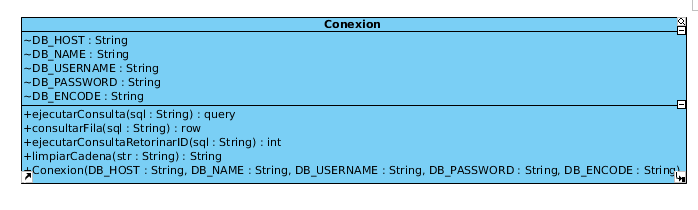
\includegraphics[width=.5\textwidth]{tlato-images/conexion}}
    		\caption{Clase de Conexion}
    		\label{fig:conexion}
    	\end{center}
    \end{figure}
    
    En esta figura ~\ref{fig:conexion} se muestran las clases del objeto de conexión, el cual contiene toda la información necesaria para conectarse a la base de Datos, así como las instrucciones principales de consulta de información y limpieza de datos para evitar inyecciones SQL y ataques XSS.
    
    \subsection{Clases del modelo Datos.Tabla}
    
    \begin{figure}[htbp!]
    	\begin{center}
    		\fbox{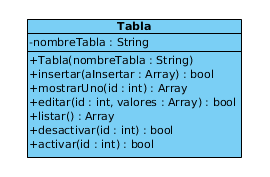
\includegraphics[width=.5\textwidth]{tlato-images/tabla}}
    		\caption{Clases dentro del paquete Datos.Tabla}
    		\label{fig:tabla}
    	\end{center}
    \end{figure}
    
    En la figura~\ref{fig:tabla} se observa la generlización de muchas de las tablas abordadas posteriormente en Modelos. \\
    El Objeto Tabla, como ya se dijo, contiene la generalización de las acciones que abordarán otros objetos, como lo son insertar, editar, activar, desactivar, mostrar y consultar, las cuales se aplican casi a cualquier tabla corriendo sobre nuestra plataforma. \\
    
    \subsection{Clases del modelo Datos.Modelos}
    
    \begin{figure}[htbp!]
    	\begin{center}
    		\fbox{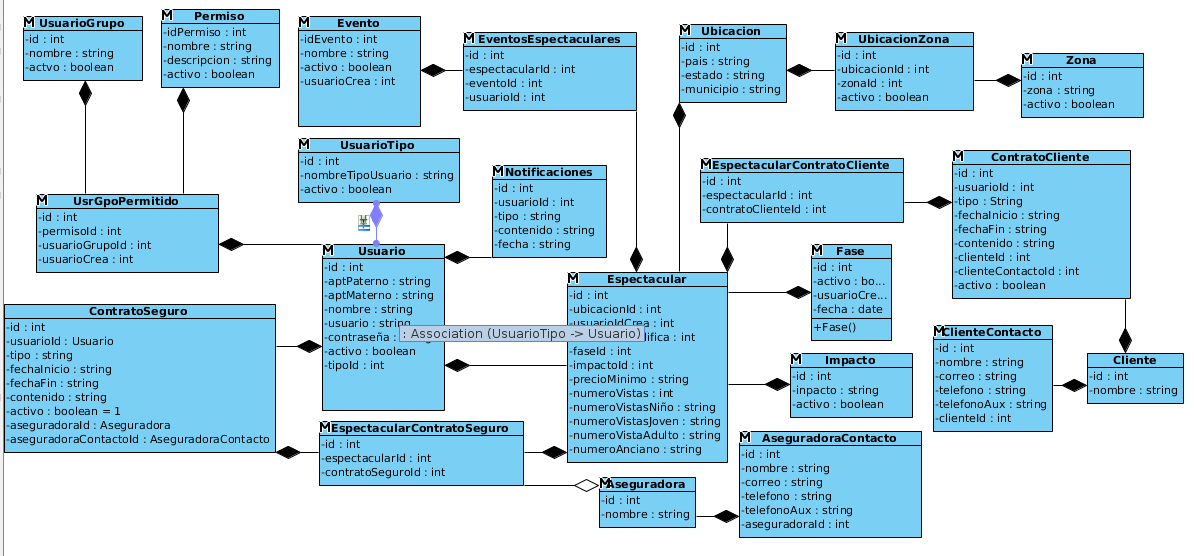
\includegraphics[width=.7\textwidth]{tlato-images/modelos}}
    		\caption{Estructura del paquete Modelos}
    		\label{fig:modelos}
    	\end{center}
    \end{figure}
    
    En la figura~\ref{fig:modelos} se describe la estructura del subsistema Datos.Modelos, la cual tiene múltiples clases para manejar personalizadamente el acceso a los datos, encargándose de procesar peticiones de la capa de Negocio y buscar o enviar información directamente hacia un medio persistente, genera arreglos u objetos dependiendo de cómo esté configurado el tipo de retorno de la clase en cuestión, y todas ellas heredan de la clase Tabla, que contiene las operaciones básicas por tabla.
    
    \subsection{Clases del modelo Negocio.Op\_generales}
    
    \begin{figure}[htbp!]
    	\begin{center}
    		\fbox{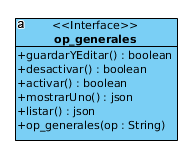
\includegraphics[width=.3\textwidth]{tlato-images/op_generales}}
    		\caption{Estructura del paquete de operaciones Generales}
    		\label{fig:op_generales}
    	\end{center}
    \end{figure}
    
    En esta figura~\ref{fig:op_generales} se desarrolla una generalización de las operaciones que pueden ser realizadas por la api, mostrando los métodos de retorno (siempre JSON o un booleano). 
    
    \subsection{Clases del modelo Negocio.Api}
    
    \begin{figure}[htbp!]
    	\begin{center}
    		\fbox{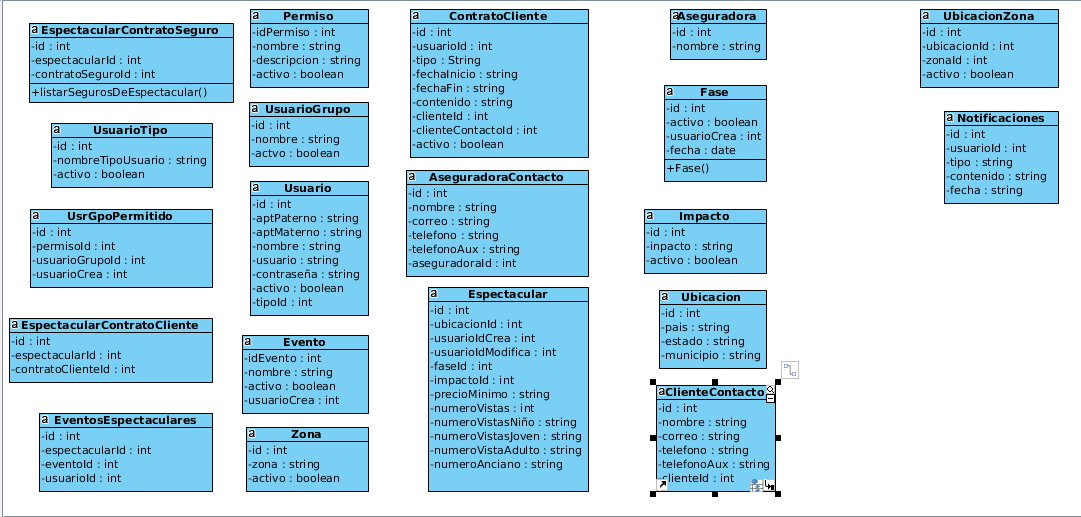
\includegraphics[width=.7\textwidth]{tlato-images/api}}
    		\caption{Estructura del modulo Api}
    		\label{fig:api}
    	\end{center}
    \end{figure}
    
    En la figura~\ref{fig:api} se muestran todas las clases que manejan información, recibiendo peticiones de la vista y mostrandole JSON de vuelta. Las clases en este módulo tienen una relación 1:1 con las clases en Datos.Modelo, debido a que cada parte de consulta tiene también su parte de manejo de datos con el mismo nombre. Además, se tienen atributos con los nombres en la base de datos debido a que las peticiones, ya sea via GET o POST llevan los nombres de dichos campos de la tabla. Se recibe el valor si está seteado y NULL si no lo está, y la variable operacional "op" será la que indique en cada ocasión la operación que ha de realizarse. 
    
    \subsection{Clases del modelo Presentacion.Componentes}
    
    \begin{figure}[htbp!]
    	\begin{center}
    		\fbox{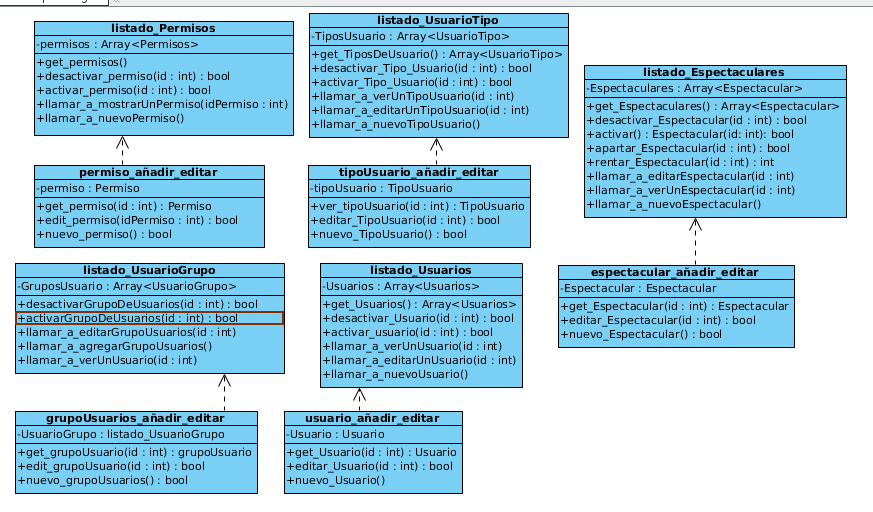
\includegraphics[width=.7\textwidth]{tlato-images/componentes}}
    		\caption{Estructura del modulo de Componentes(vistas)}
    		\label{fig:componentes}
    	\end{center}
    \end{figure}
    
    En la figura~\ref{fig:componentes} se muestra el orientado a Componentes que manejaremos, en el cual cada componente de la vista realiza solo la tarea que necesita realizar, no manejándolos por vistas sino, repitiendo, por componentes. Cada componente tendrá su propio html, css y JS incorporado, y manejará solo los datos correspondientes a si mismo en la API. Generalmente, a menos que requiera funcionalidad adicional, cada clase de la API solo contará con dos componentes, uno para listado, activación y desactivación, y otro para mostrar un único registro, o editarlo. Se aprovechó también el hecho de que para insertar o editar un registro, sólo cambia el ID, lo que facilita el diseño(si un registro tiene ID, significa que está registrado y hay que editarlo, en caso contrario, es nuevo y hay que registrarlo).
    
%	El alcance funcional del sistema se describe en esta sección especificando la prioridad como:
%	
%\begin{description}
%	\item[MA:] Muy alta.
%	\item[A:] Alta.
%	\item[M:] Media.
%	\item[B:] Baja.
%	\item[MB:] Muy baja.
%\end{description}

%	En este caso la prioridad describe el grado de importancia (Relevancia y urgencia) que tiene para el negocio que el sistema cumpla con dicho requerimiento.

%% - - - - - - - - - - - - - - - - - - - - - - - - - - - - - 
%\subsection{Requerimientos del usuario}
%
%\begin{table}[hbtp!] 
%    \begin{cdtUsrRequirements}[author=Ulises Vélez Saldaña, revisor=Juan Pérez, status=\cdtStRevision]
%    	\RUitem{RU1}{Gestión de vehículos}{El sistema deberá facilitar el llevar un registro actualizado de los vehículos con los que cuenta la empresa.}
%    	\RUitem{RU2}{...}{...}
%    \end{cdtUsrRequirements}
%	\caption{Requerimientos del usuario.}
%	\label{tbl:requerimientosUsuario}
%\end{table}
%
%% - - - - - - - - - - - - - - - - - - - - - - - - - - - - - 
%\subsection{Requerimientos del sistema}
%
%\begin{table}[htpb!]
%    \begin{cdtRequirements}[author=Ulises Vélez Saldaña, revisor=Juan Pérez, status=\cdtStRevision]
%    	\RFitem{RF1}{Gestión de vehículos}{El sistema deberá facilitar el llevar un registro actualizado de los vehículos con los que cuenta la empresa.}{A}{RU1}
%    	\RFitem{RF2}{...}{...}{}{}
%    \end{cdtRequirements}
%	\caption{Requerimientos del sistema.}
%	\label{tbl:requerimientosSistema}
%\end{table}





